\documentclass[8pt]{beamer}

\title{Accélération Python avec GPU}
\subtitle{Présentation de TAL}
\author{Joseph Leonard Stephen Auguste}
\usetheme{Goettingen}

\usepackage[utf8]{inputenc}
\usepackage[french]{babel}
\usepackage[T1]{fontenc}
\usepackage{hyperref}
\usepackage{listings}
\usepackage{graphicx}
\usepackage{dirtytalk}
\usepackage{xcolor}
\usepackage{lstautogobble}

\addtobeamertemplate{navigation symbols}{}{%
    \usebeamerfont{footline}%
    \usebeamercolor[fg]{footline}%
    \hspace{1em}%
    \insertframenumber/\inserttotalframenumber{}
}

\definecolor{codegreen}{rgb}{0,0.6,0}
\definecolor{codegray}{rgb}{0.5,0.5,0.5}
\definecolor{codepurple}{rgb}{0.58,0,0.82}
\definecolor{backcolour}{rgb}{0.95,0.95,0.92}

\lstdefinestyle{mystyle}{
    backgroundcolor=\color{backcolour},   
    commentstyle=\color{codegreen},
    keywordstyle=\color{magenta},
    numberstyle=\tiny\color{codegray},
    stringstyle=\color{codepurple},
    basicstyle=\ttfamily\footnotesize,
    breakatwhitespace=false,         
    breaklines=true,                 
    captionpos=b,                    
    keepspaces=true,                 
    numbers=left,                    
    numbersep=5pt,                  
    showspaces=false,                
    showstringspaces=false,
    showtabs=false,                  
    tabsize=2,
    belowskip=-0.5em,
    autogobble
}

\lstset{style=mystyle}


\begin{document}

\maketitle

\section{Introduction}
\begin{frame}
    \frametitle{Les outils}
    \say{OpenCL (Open Computing Language) est la combinaison d'une API 
    et d'un langage de programmation dérivé du C, 
    proposé comme un standard ouvert par le Khronos Group.}
    \newline
    \-- Wikipédia\pause{}
    \vspace{20pt}
    \newline
    OpenCL permet:\pause{}
    \begin{itemize}
        \item Programmer sur GPU\pause{}
        \item Parallélisation:
            \begin{itemize}
                \item Parallélisation de tâches \textit{(task parallelism)}
                \item Parallélisation de données \textit{(data parallelism)}
            \end{itemize}
    \end{itemize}\pause{}
    \vspace{20pt}
    PyOpenCL:\pause{}
    \begin{itemize}
        \item \textit{Framework} pour intégrer du code OpenCL à du code Python\pause{}
        \item Projet \textit{open source}: \url{github.com/inducer/pyopencl}
    \end{itemize}\pause{}
    \vspace{20pt}
    Code présenté: \url{github.com/leonardSA/gpu_python_acceleration}
\end{frame}




\section{Introduction à OpenCL}
\begin{frame}
    \frametitle{Introduction à OpenCL}  

    Couche d'abstraction matériel: cibler GPU, CPU et FPGA\pause{}
    \vspace{10pt}

    Programme hôte (Python)\pause{}

    Kernels:\pause{}
    \begin{itemize}
        \item Dérivé du C99\pause{}
        \item Fonctionnalités enlevées:\pause{}
            \begin{itemize}
                \item Récursivité
                \item Pointeurs de fonctions
                \item Allocation dynamique
                \item \textit{bit fields}
            \end{itemize}\pause{}
        \item Fonctionnalités ajoutées:\pause{}
            \begin{itemize}
                \item Types spéciaux e.g. \textit{float4}
                \item Fonctions spéciales e.g. \textit{barrier}
            \end{itemize}
    \end{itemize}\pause{}
    \vspace{10pt}

    Opérations sont des événements

    Opérations placées dans une file d'exécution: \textit{queue}\pause{}
    \vspace{10pt}

    Plusieurs modèles à comprendre:\pause{}
    \begin{itemize}
        \item modèle d'exécution
        \item modèle de mémoire
    \end{itemize}
\end{frame}

\begin{frame}
    \frametitle{Modèle d'exécution}

    \textit{NDRange}: \textit{N-dimensions range}\pause{}
    \begin{itemize}
        \item \textit{Global NDRange}: G
        \item \textit{Local NDRange}: L
    \end{itemize}\pause{}
    
    Au lancement d'un Kernel:
    \begin{itemize}
        \item \textit{work item}:\pause{} 
            \begin{itemize}
                \item ${\displaystyle nombre(\textrm{work items}) = \prod_{i=0}^{N}G[i]}$\pause{}
                \item exécute le kernel
                \item exécution concurrente
            \end{itemize}

        \item \textit{work group}:\pause{}
            \begin{itemize}
                \item regroupe les \textit{work items}\pause{}
                \item ${\displaystyle nombre(\textrm{work groups}) = nombre(\textrm{work items}) /
                    \prod_{i=0}^{N}L[i]}$\pause{}
                \item exécution parallèle
                \item exécuté par les \textit{compute units}
            \end{itemize}
    \end{itemize}
\end{frame}

\begin{frame}
    \frametitle{Modèle d'exécution}
    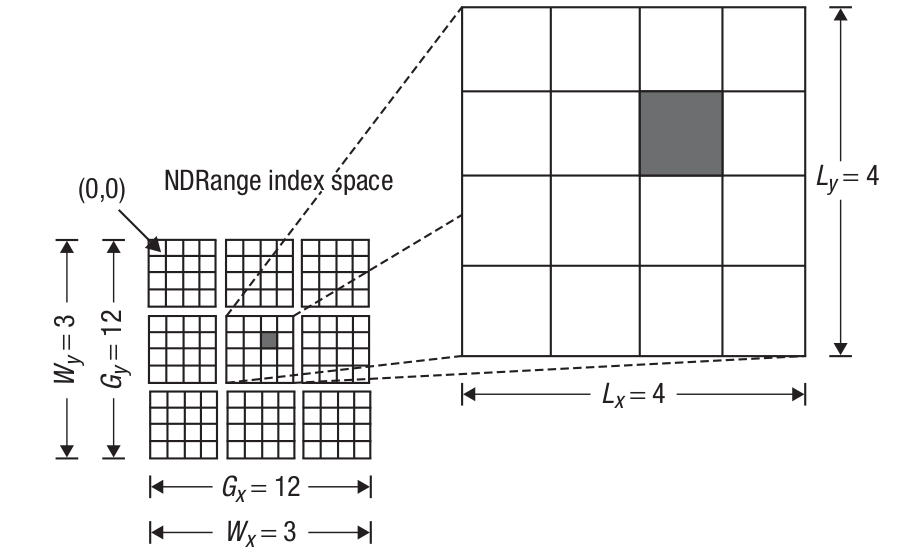
\includegraphics[width=\textwidth]{../resources/execution_model.png}
\end{frame}

\begin{frame}
    \frametitle{Modèle de mémoire}
    \textit{Memory objects}:\pause{}
    \begin{itemize}
        \item \textit{buffer objects}
        \item \textit{image objects}
    \end{itemize}\pause{}
    \vspace{20pt}

    5 régions de mémoire:\pause{}
    \begin{itemize}
        \item \textit{host memory}: accessible uniquement par l'hôte\pause{}
        \item \textit{global memory}: accessible par tous\pause{}
        \item \textit{constant memory}: comme la mémoire globale mais constante\pause{}
        \item \textit{local memory}: lié à un \textit{work group}\pause{}
        \item \textit{private memory}: lié à un \textit{work item}
    \end{itemize}
\end{frame}

\begin{frame}
    \frametitle{Modèle de mémoire}
    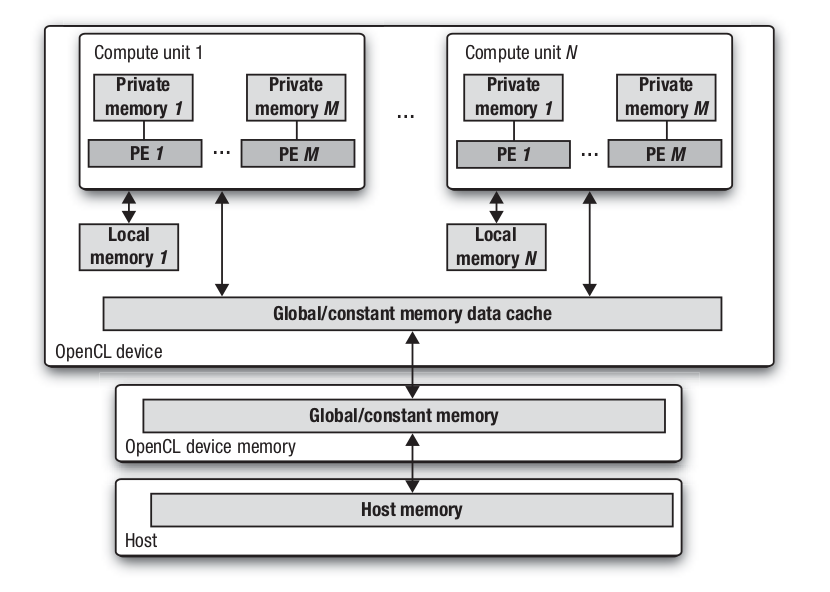
\includegraphics[width=\textwidth]{../resources/memory_model.png}
\end{frame}


\section{Implémentation naïve de la multiplication de matrices}
\begin{frame}[fragile]
    \frametitle{Implémentation naïve de la multiplication de matrices}
    Principe:
    \[
        C_{ij} = \sum_{k=1}^{n} a_{ik}b_{kj}\quad\textrm{pour}\quad i = 1, \dots, m\quad \textrm{et}\quad j = 1,\dots,p
    \]\pause{}

    Pour exécuter il faut configurer créer le contexte d'exécution:\pause{}
    \begin{lstlisting}[language=Python]
    import pyopencl as cl
    # choose first platform 
    platform = cl.get_platforms()[0]       
    # retrieve platform devices to create context
    devices = platform.get_devices()        
    # create context for platform
    context = cl.Context(devices=devices)    
    # add OpenCL source code to context (source is a string)
    program_source = cl.Program(context, source)
    # compile the kernel
    program = program_source.build()
    # create the command queue for the context => make the builded programs avaiable for execution
    queue = cl.CommandQueue(context)
    \end{lstlisting}
\end{frame}

\begin{frame}[fragile]
    \frametitle{Implémentation naïve de la multiplication de matrices}
    Définition du kernel \textit{(program\_source)}:
    \begin{lstlisting}[language=c]
    __kernel void matrix_mult(__global float *a,
                              __global float* b,
                              __global float* c,
                              const unsigned int a_ncol,
                              const unsigned int b_ncol) {
        int rows = get_global_id(0);    /* iterate over rows */
        int columns = get_global_id(1); /* then iterate over columns */

        /* compute value */
        float value = 0;
        for (unsigned int i = 0 ; i < a_ncol ; i++) {
            value += a[rows * a_ncol + i] * b[i * b_ncol + columns];
        }

        c[rows * b_ncol + columns] = value;
    }
    \end{lstlisting} 
\end{frame}

\begin{frame}[fragile]
    \frametitle{Implémentation naïve de la multiplication de matrices}
    \begin{lstlisting}[language=python]
    import numpy as np
    import pyopencl as cl

    # a_dim is a tuple with (row, column) for A
    A = np.random.rand(A_dim[0] * A_dim[1]).astype(np.float32)   
    # b_dim ditto
    B = np.random.rand(B_dim[0] * B_dim[1]).astype(np.float32)   
    C = np.zeros(A_dim[1] * B_dim[0], dtype=np.float32)

    A_buffer = cl.Buffer(context, flags=cl.mem_flags.READ_ONLY, size=A.nbytes)
    B_buffer = cl.Buffer(context, flags=cl.mem_flags.READ_ONLY, size=B.nbytes)
    C_buffer = cl.Buffer(context, flags=cl.mem_flags.WRITE_ONLY, size=C.nbytes)

    cl.enqueue_copy(queue, src=A, dest=A_buffer)
    cl.enqueue_copy(queue, src=B, dest=B_buffer)

    kernel_arguments = (A_buffer, B_buffer, C_buffer, A_dim[1], B_dim[1])
    # .wait() to wait for the event to finish
    program.matrix_mult(queue, 
                       [A_dim[0], B_dim[1]],     # global dimensions
                       None, 
                       *kernel_arguments).wait()

    cl.enqueue_copy(queue, src=C_buffer, dest=C)
    \end{lstlisting}
\end{frame}

\begin{frame}
    \frametitle{Implémentation naïve de la multiplication de matrices}
    Trois genres de mesures:\pause{}
    \begin{itemize}
        \item le temps de copie des \textit{buffers}\pause{}
        \item le temps d'exécution\pause{}
        \item la précision des résultats\pause{}
    \end{itemize}\pause{}
    \vspace{20pt}
    Des matrices carrées de même dimension allant de 10 à 1 500 lignes/colonnes par pas de 10.
\end{frame}

\begin{frame}
    \frametitle{Implémentation naïve de la multiplication de matrices}
    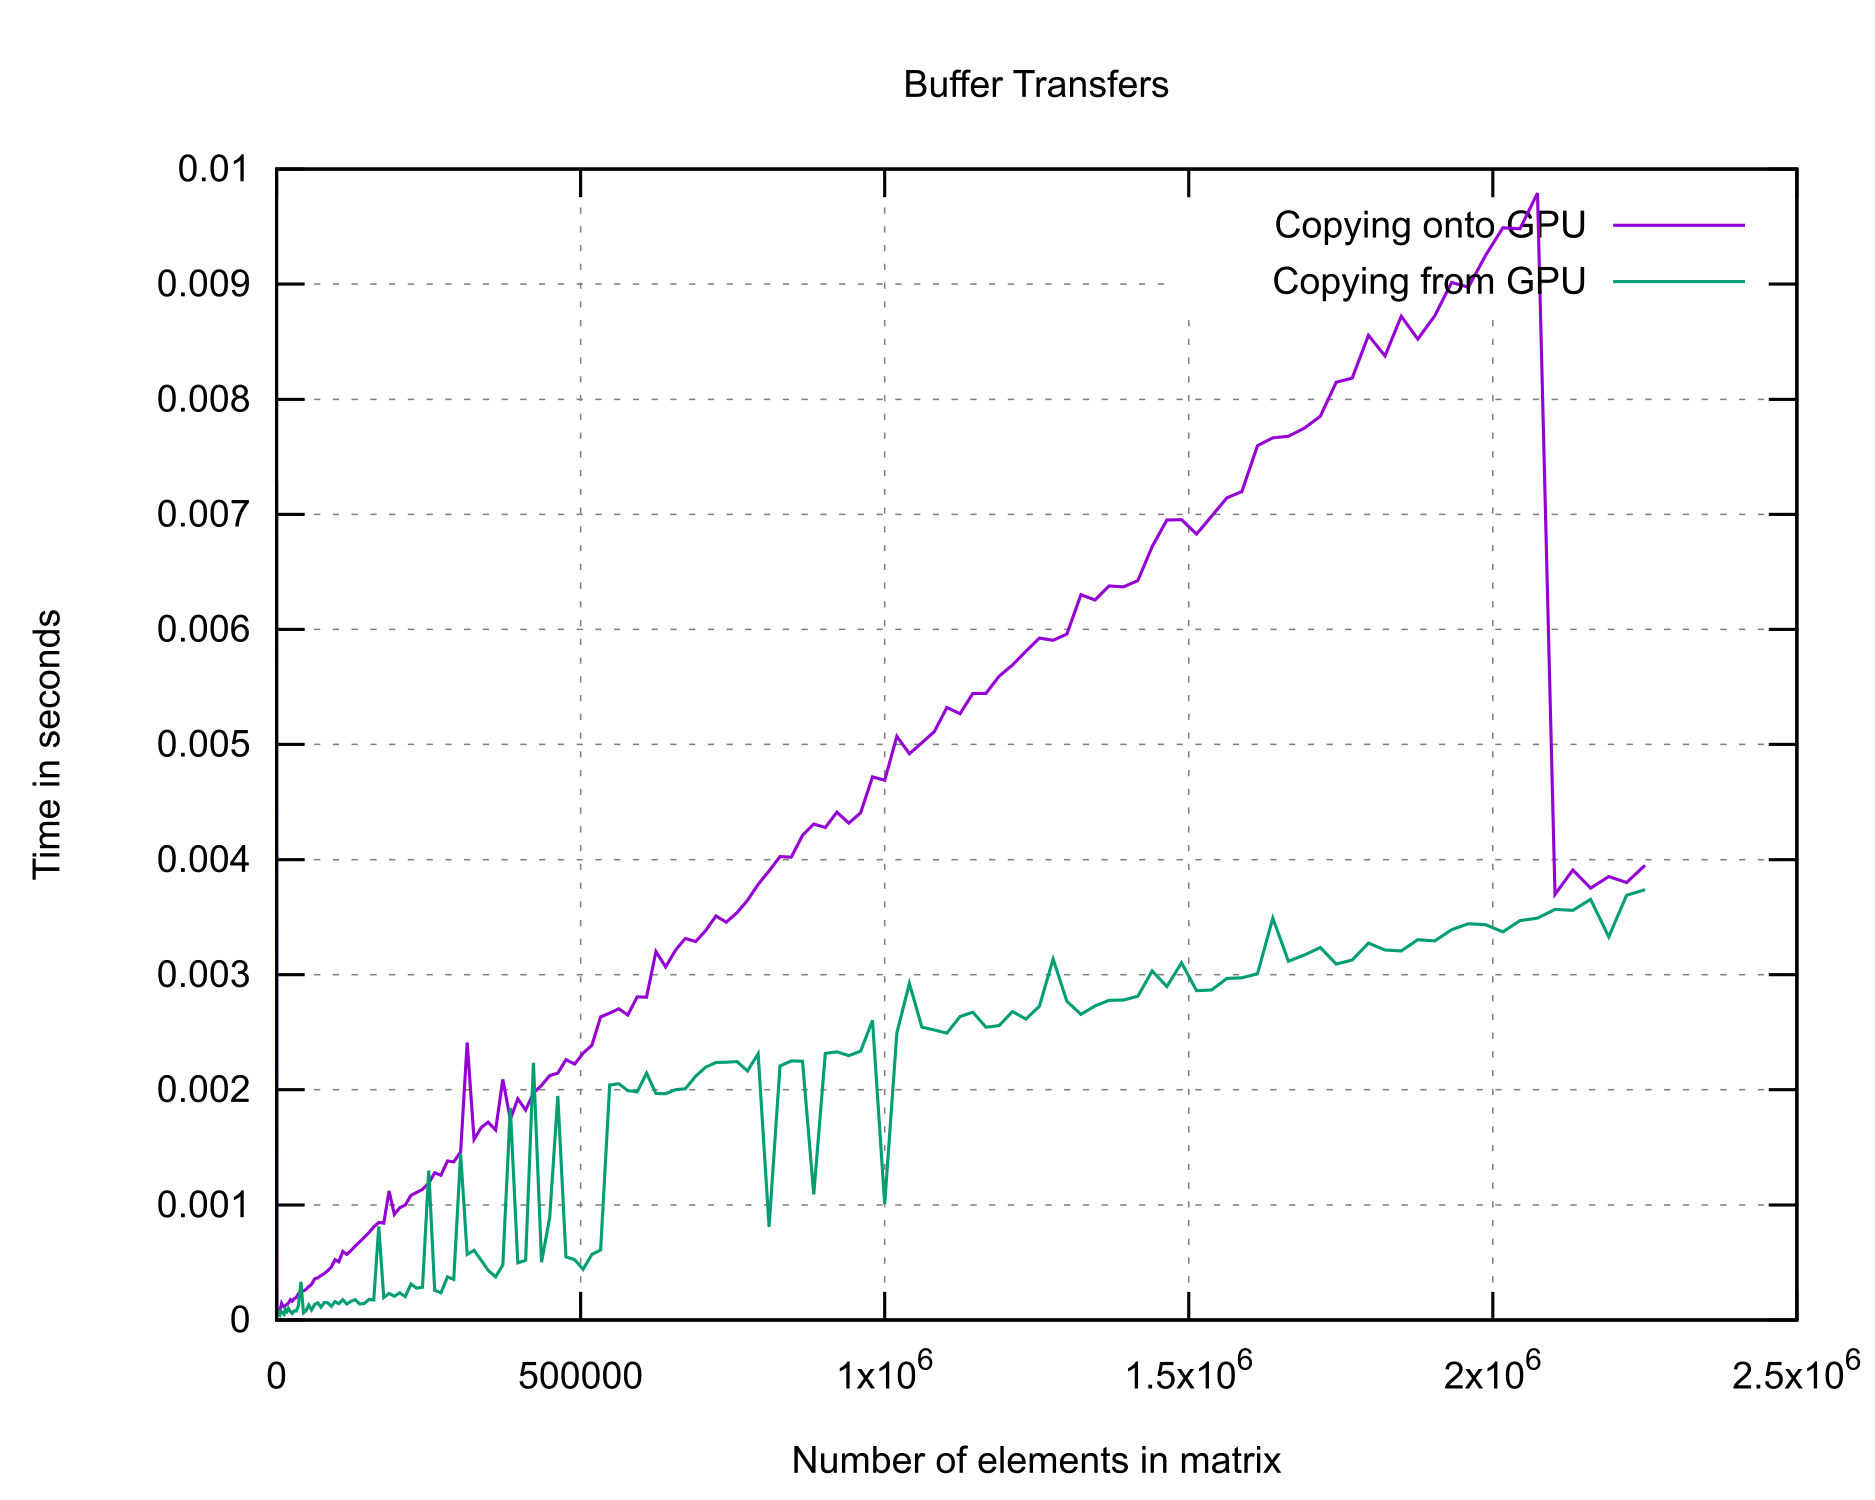
\includegraphics[width=\textwidth]{../resources/matrix_naive_buffer_transfer.png}
\end{frame}

\begin{frame}
    \frametitle{Implémentation naïve de la multiplication de matrices}
    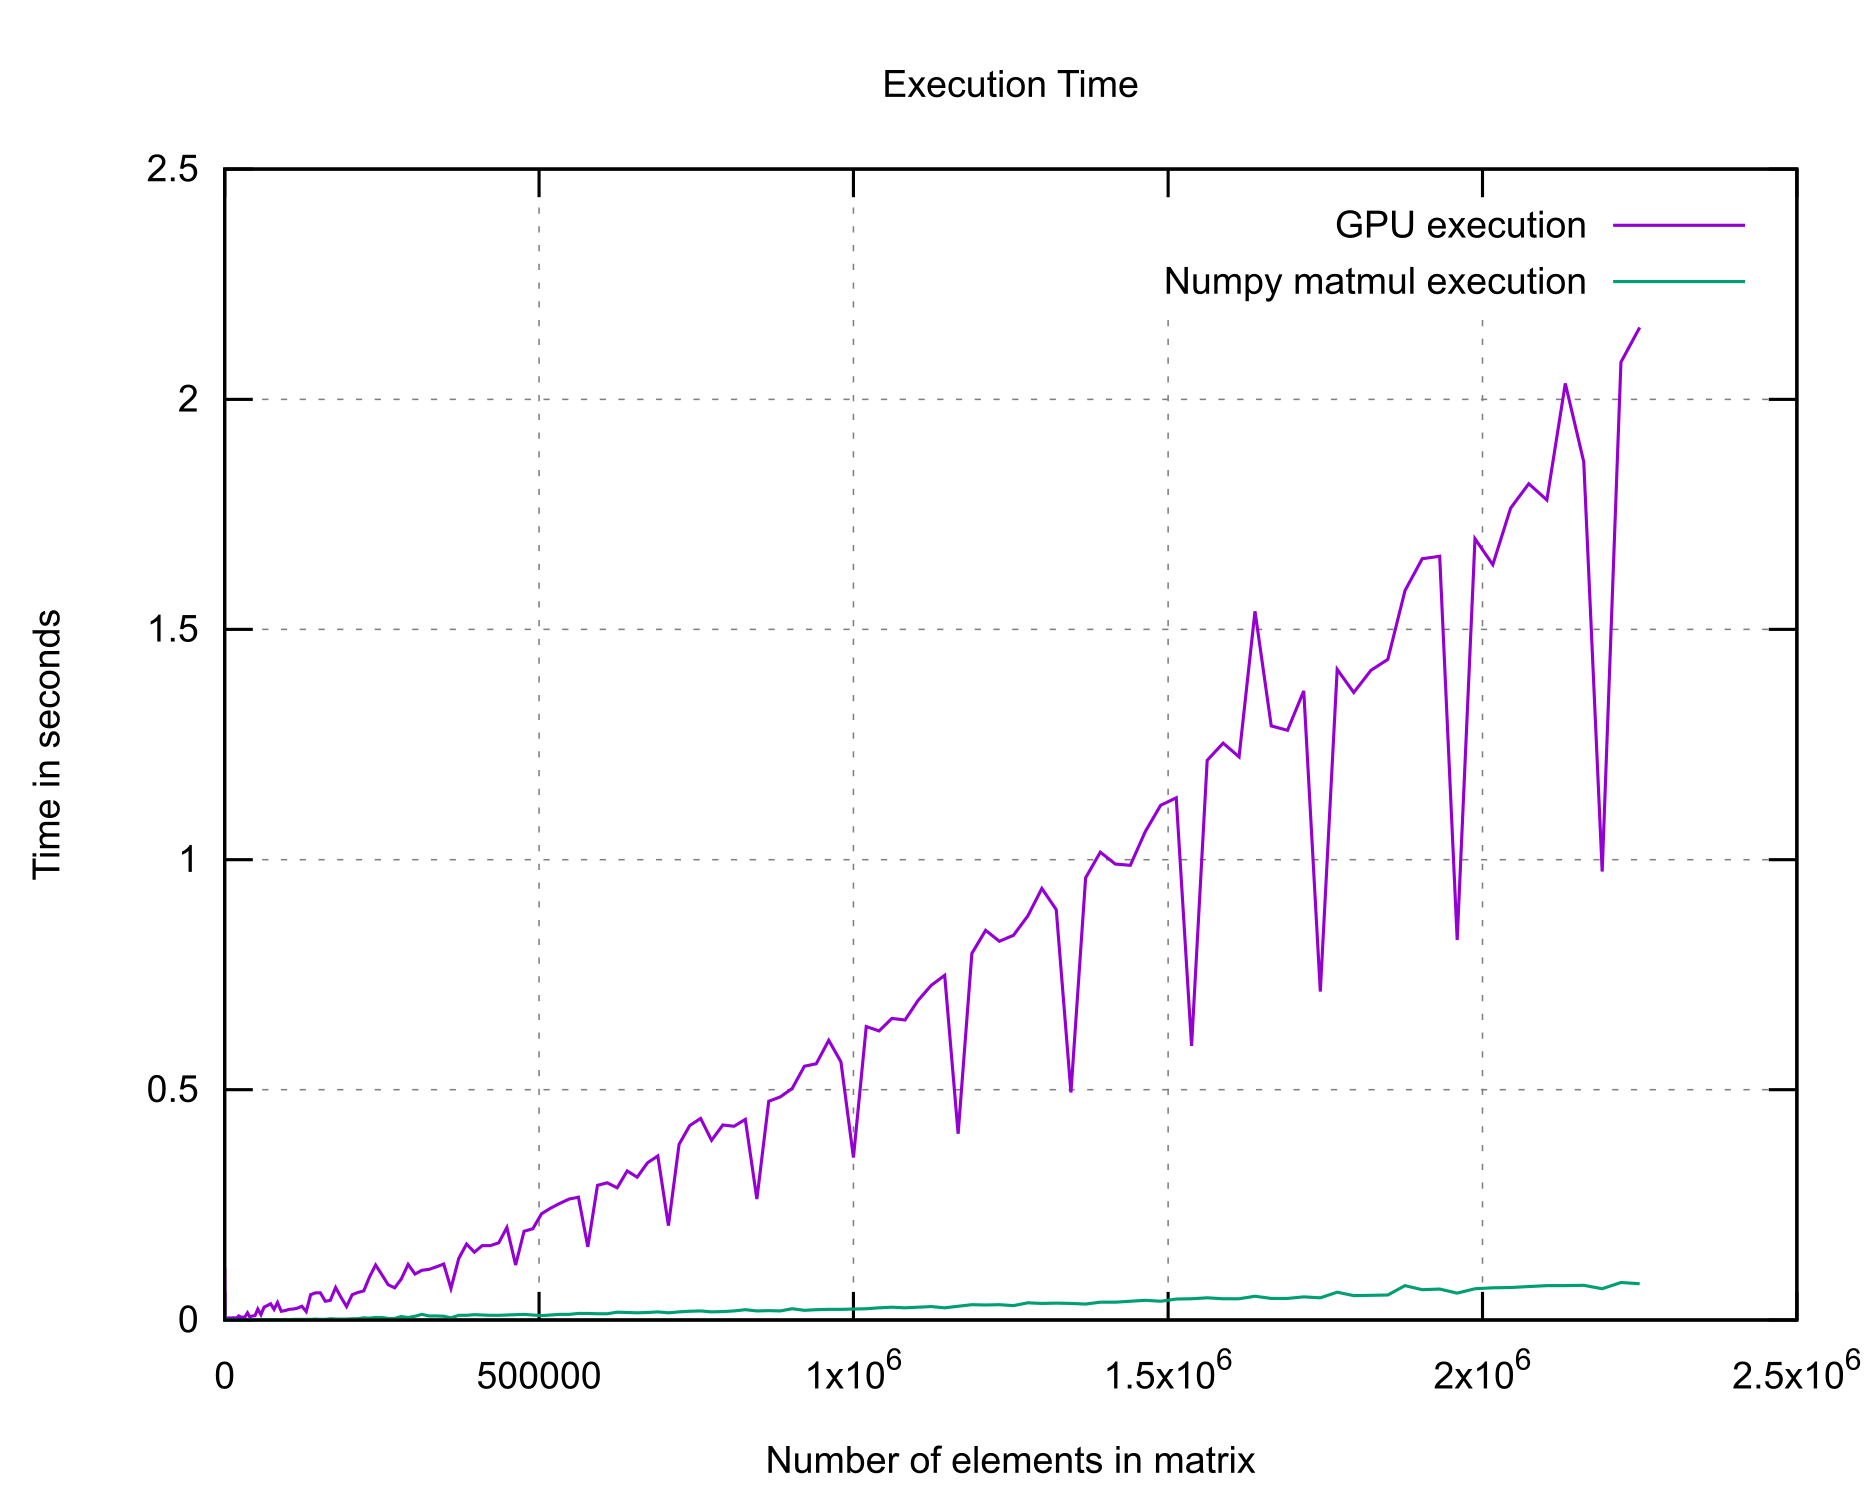
\includegraphics[width=\textwidth]{../resources/matrix_naive_execution_time.png}
\end{frame}

\begin{frame}
    \frametitle{Implémentation naïve de la multiplication de matrices}
    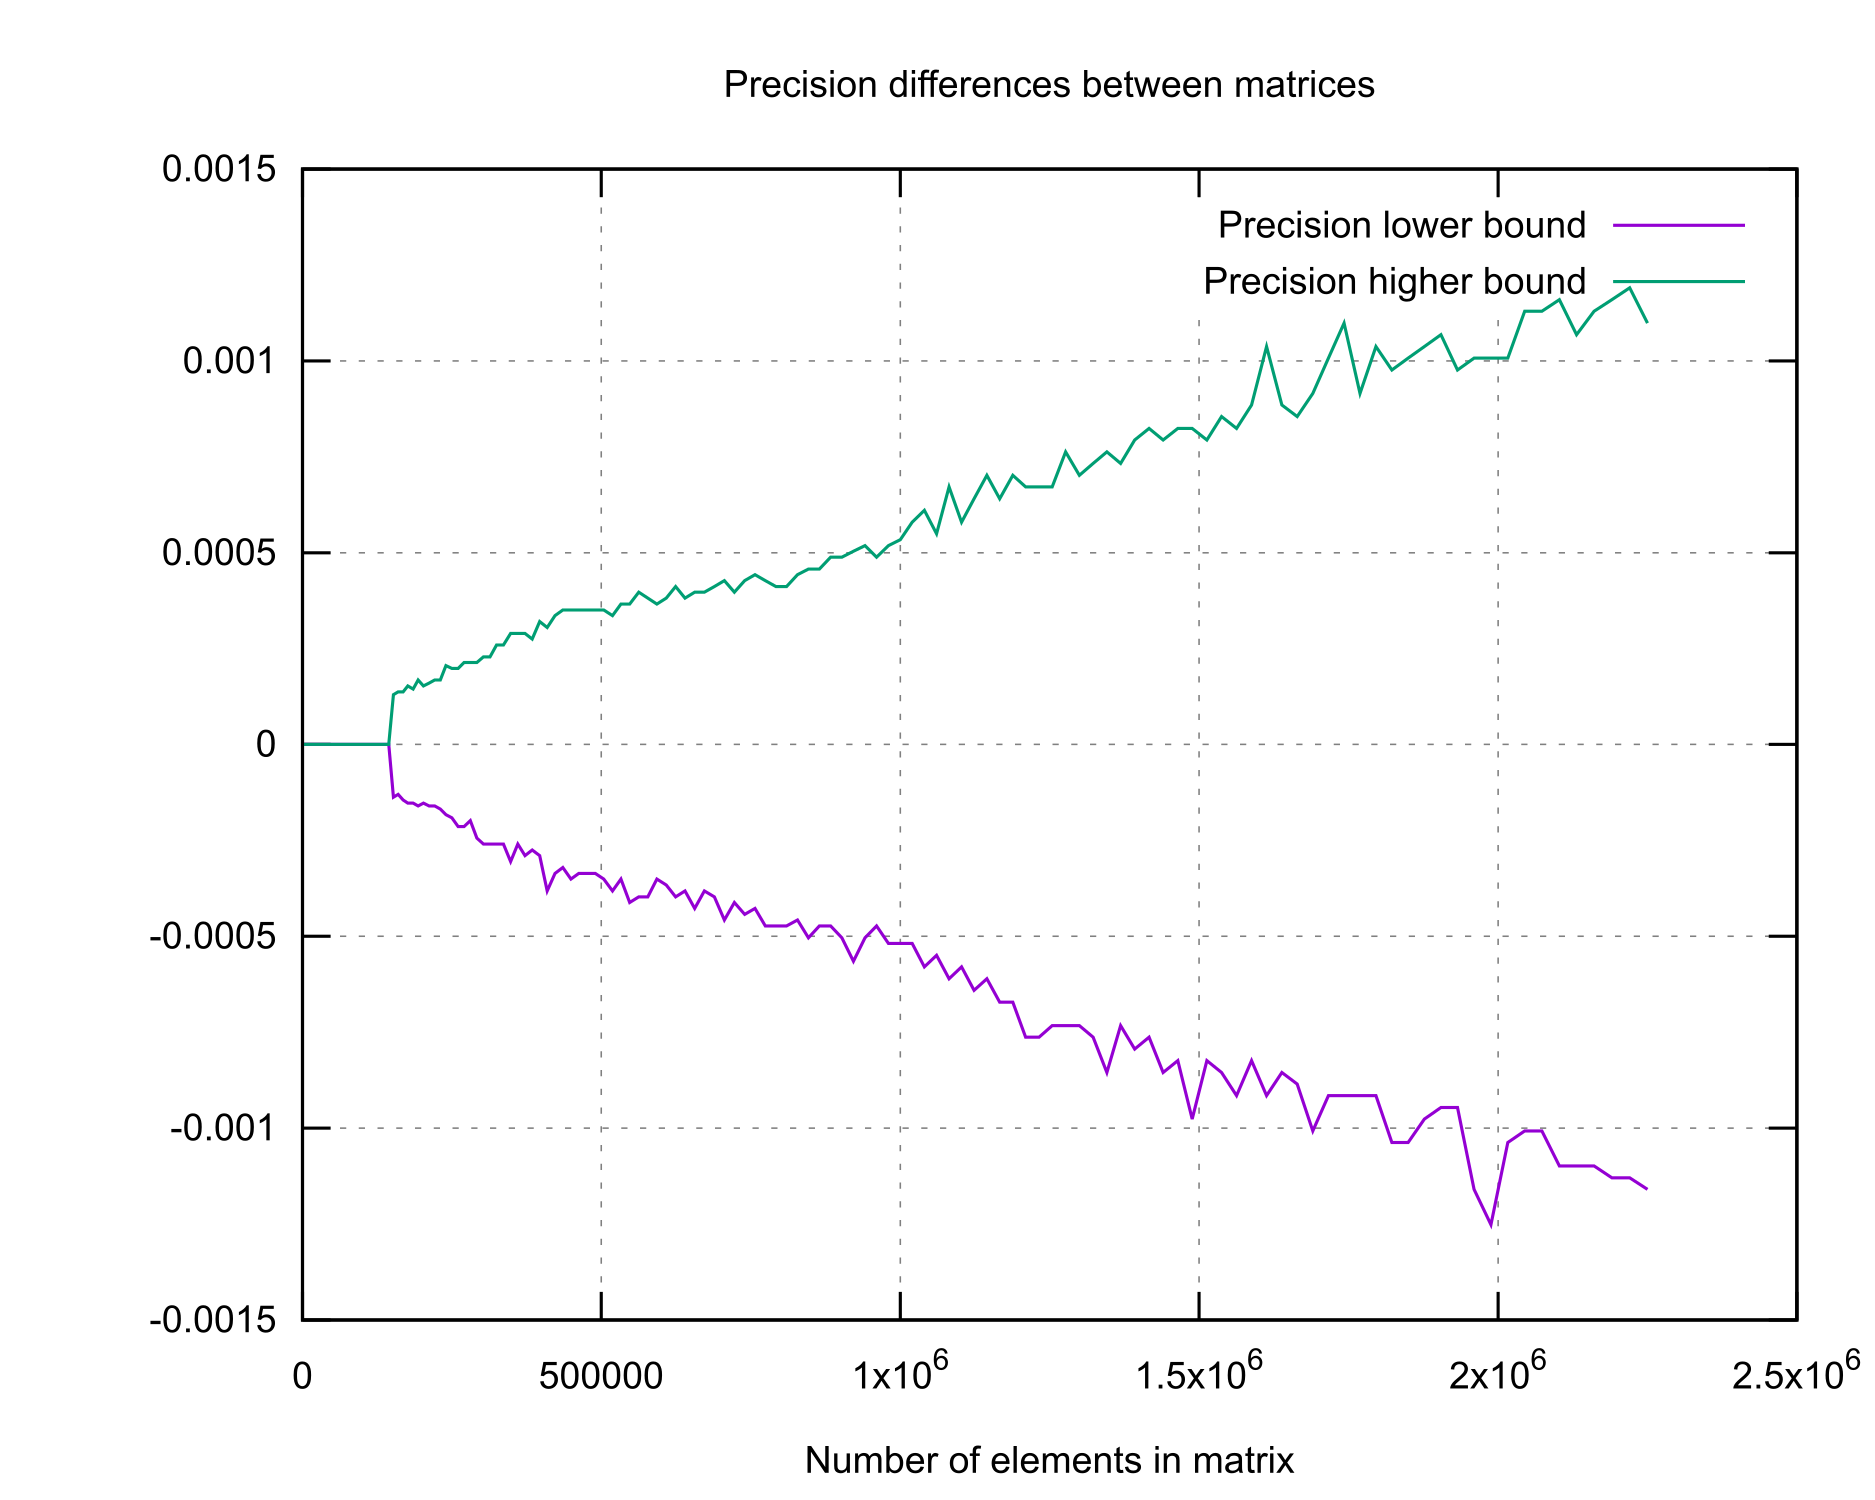
\includegraphics[width=\textwidth]{../resources/matrix_naive_float_precision.png}
\end{frame}

\begin{frame}
    \frametitle{Implémentation naïve de la multiplication de matrices}
    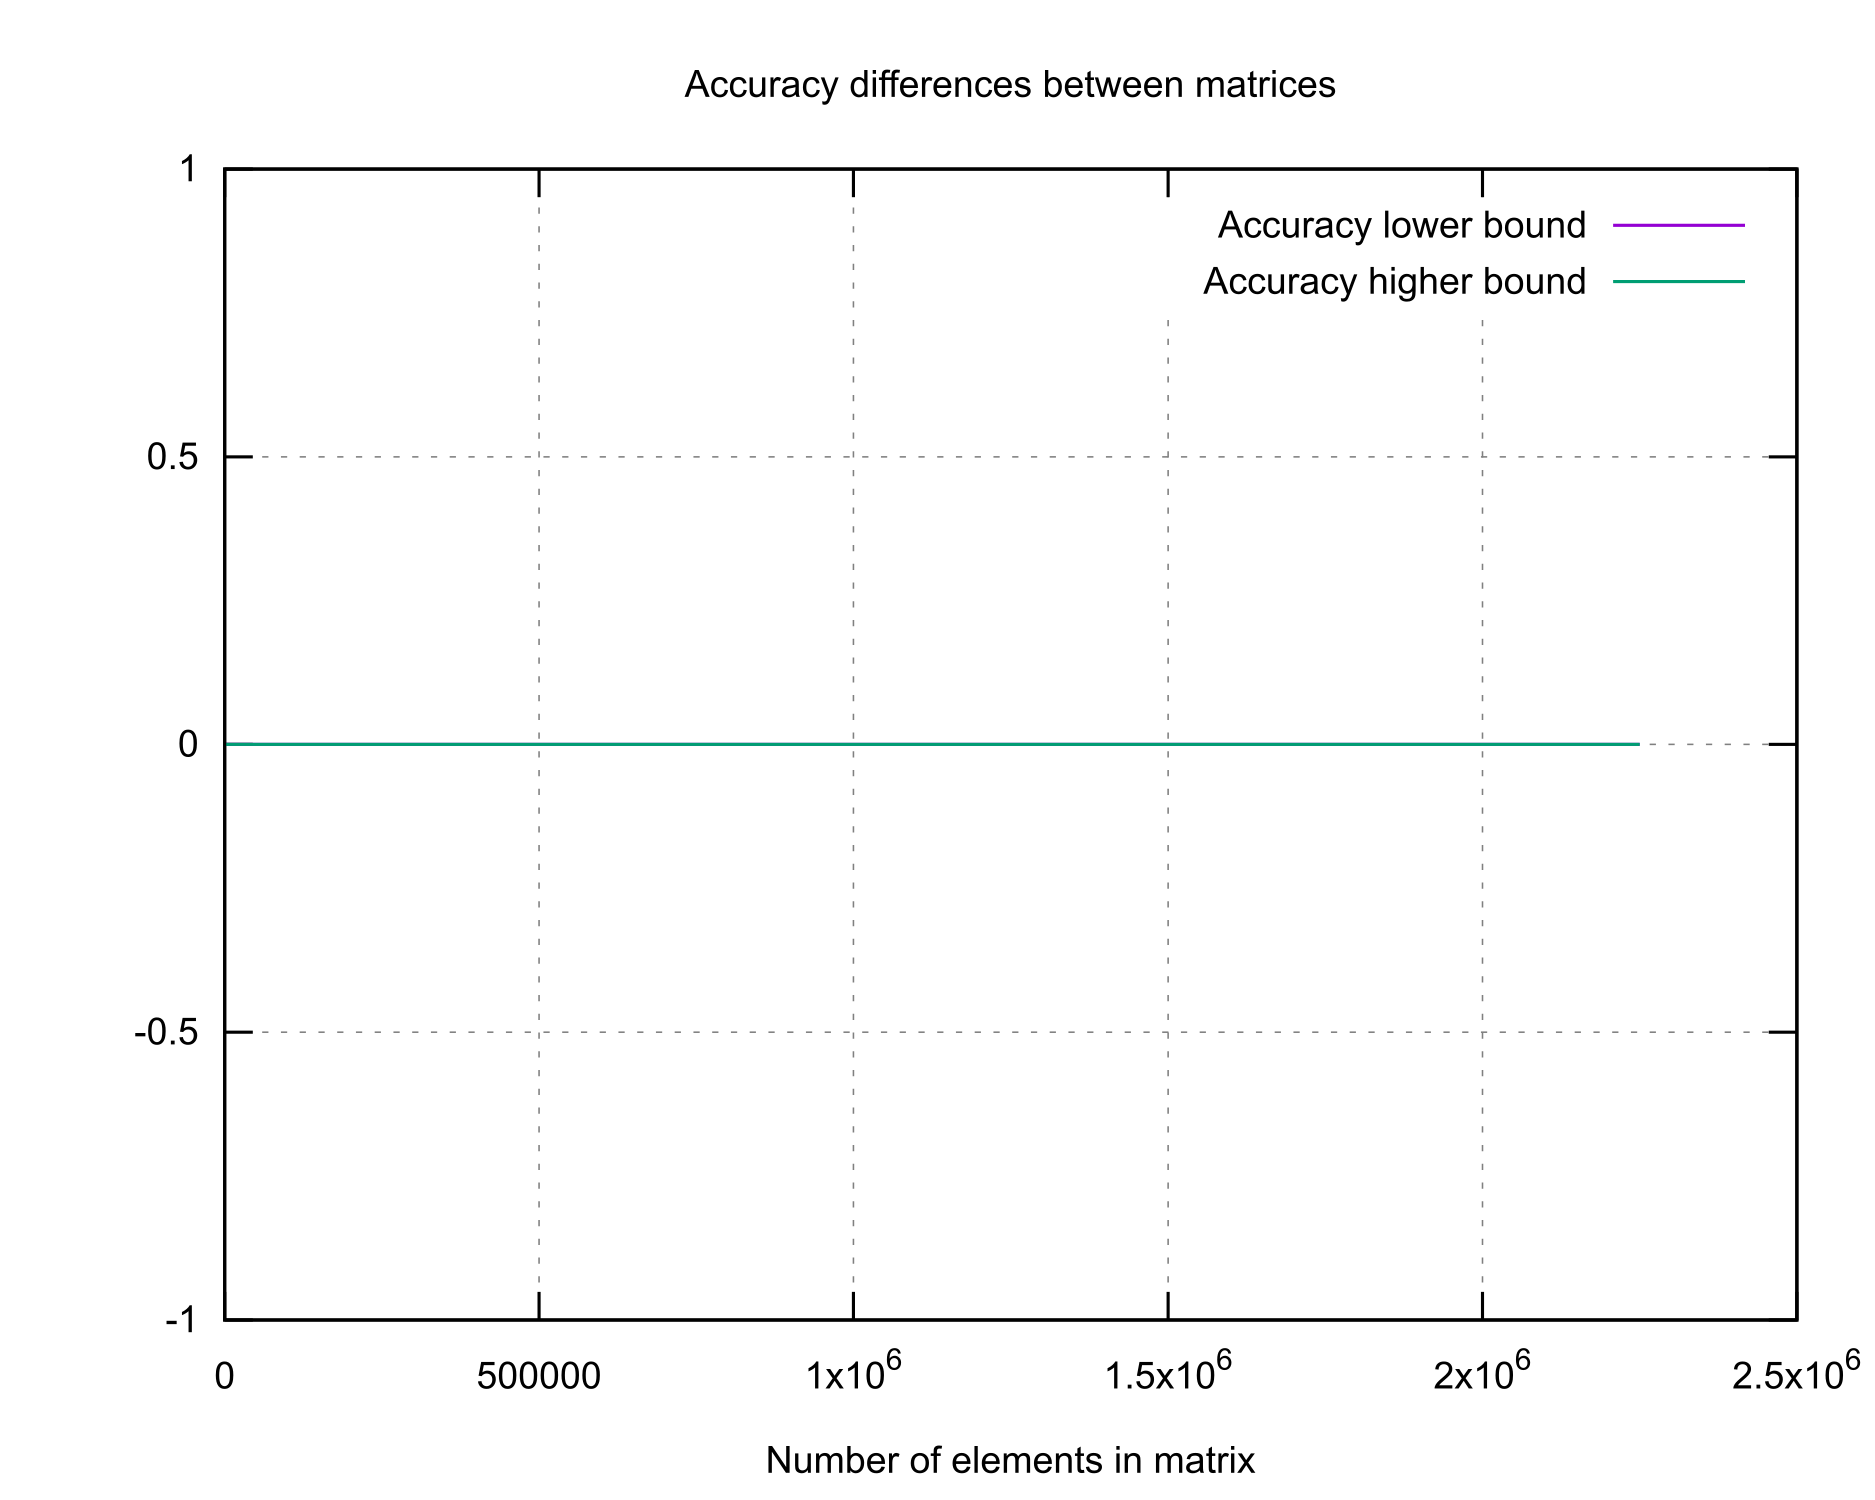
\includegraphics[width=\textwidth]{../resources/naive_integer_accuracy.png}
\end{frame}


\section{Implémentation non naïve de la multiplication de matrices}
\begin{frame}
    \frametitle{Implémentation non naïve de la multiplication de matrices}
    Implémentation tirée du livre \textit{OpenCL Programming Guide}.
    \newline
    Principe:\pause{}
    \begin{itemize}
        \item un \textit{work item} calcule une ligne de la matrice C\pause{}
        \item les \textit{work items} sont regroupés dans différents \textit{work groups}\pause{}
    \end{itemize}
    But: optimiser les mouvements de données.\pause{}
    \vspace{10pt}
    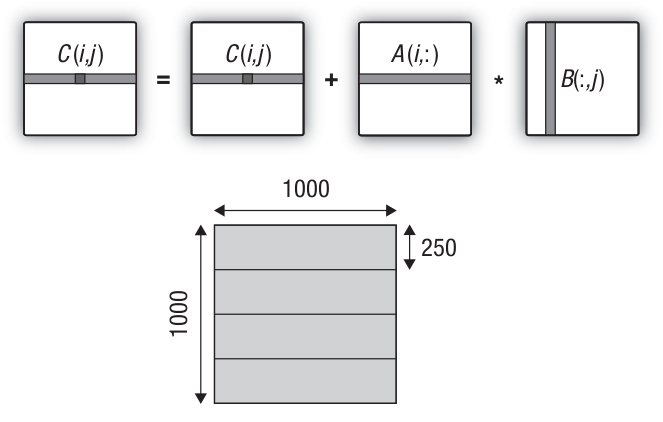
\includegraphics[width=\textwidth]{../resources/non_naive_implementation_principle.png}
\end{frame}

\begin{frame}[fragile,allowframebreaks]
    \frametitle{Implémentation non naïve de la multiplication de matrices}
    \begin{lstlisting}[language=python]
    import numpy as np
    import pyopencl as cl

    N_WORK_GROUPS = 32
    # we keep size which represents a lenght of a line/colunm 
    # by powers of two to be able to divide evenly everything for work groups
    size = next_power_of_two32bit(max([A_dim[0], A_dim[1], B_dim[0], B_dim[1]]))    

    A = np.random.rand(A_dim[0] * A_dim[1]).astype(np.float32)   
    B = np.random.rand(B_dim[0] * B_dim[1]).astype(np.float32)   
    C = np.zeros(A_dim[1] * B_dim[0], dtype=np.float32)

    # our matrices are now of dimensions (size, size)
    A = matrix_resize_with_zeros(A, size)
    B = matrix_resize_with_zeros(B, size)
    C = matrix_resize_with_zeros(C, size)

    A_buffer = cl.Buffer(context, flags=cl.mem_flags.READ_ONLY, size=A.nbytes)
    B_buffer = cl.Buffer(context, flags=cl.mem_flags.READ_ONLY, size=B.nbytes)
    C_buffer = cl.Buffer(context, flags=cl.mem_flags.WRITE_ONLY, size=C.nbytes)

    cl.enqueue_copy(queue, src=A, dest=A_buffer)
    cl.enqueue_copy(queue, src=B, dest=B_buffer)

    kernel_arguments = (A_buffer, B_buffer, C_buffer,
                        # local memory size needs to be passed for
                        # local argument
                        cl.LocalMemory(A[0].nbytes),
                        np.int32(size))

    program.matrix_mult(queue,
                        [size],
                        [size // N_WORK_GROUPS],
                        *kernel_arguments).wait()

    cl.enqueue_copy(queue, src=C_buffer, dest=C)

    matrices_resize_original_dimensions(C, A_dim[0], B_dim[1])
    \end{lstlisting}
\end{frame}

\begin{frame}[fragile]
    \frametitle{Implémentation non naïve de la multiplication de matrices}
    \begin{lstlisting}[language=c]
    /* #define AWRK_SIZE is added by the host program */
    __kernel void matrix_mult(__global float* A,
                              __global float* B,
                              __global float* C,
                              __local float* Bwrk,  /* local memory of b column for work group */
                              const int ncol) {
        int i = get_global_id(0);
        int iloc = get_local_id(0);
        int nloc = get_local_size(0);

        float Awrk[AWRK_SIZE];  /* private memory of a column for work item */

        if (i < ncol) {
            /* copy elements in private memory */
            for (int k = 0 ; k < ncol ; k++) {
                Awrk[k] = A[i * ncol + k];
            }

            for (int j = 0 ; j < ncol ; j++) {
                /* copy elements in local memory */
                for (int k = iloc ; k < ncol ; k = k + nloc) {
                    Bwrk[k] = B[k * ncol + j];
                }
                barrier(CLK_LOCAL_MEM_FENCE);
                float tmp = 0.0;
                for (int k = 0 ; k < ncol ; k++) {
                    tmp += Awrk[k] * Bwrk[k];
                }
                C[i * ncol + j] = tmp;
            }
        }
    }
    \end{lstlisting}
\end{frame}

\begin{frame}
    \frametitle{Implémentation non naïve de la multiplication de matrices}
    Trois genres de mesures:\pause{}
    \begin{itemize}
        \item le temps de copie des \textit{buffers}\pause{}
        \item le temps d'exécution\pause{}
        \item la précision des résultats\pause{}
    \end{itemize}\pause{}
    \vspace{20pt}
    Des matrices carrées de même dimension allant de 10 à 1 500 lignes/colonnes par pas de 10.
\end{frame}

\begin{frame}
    \frametitle{Implémentation non naïve de la multiplication de matrices}
    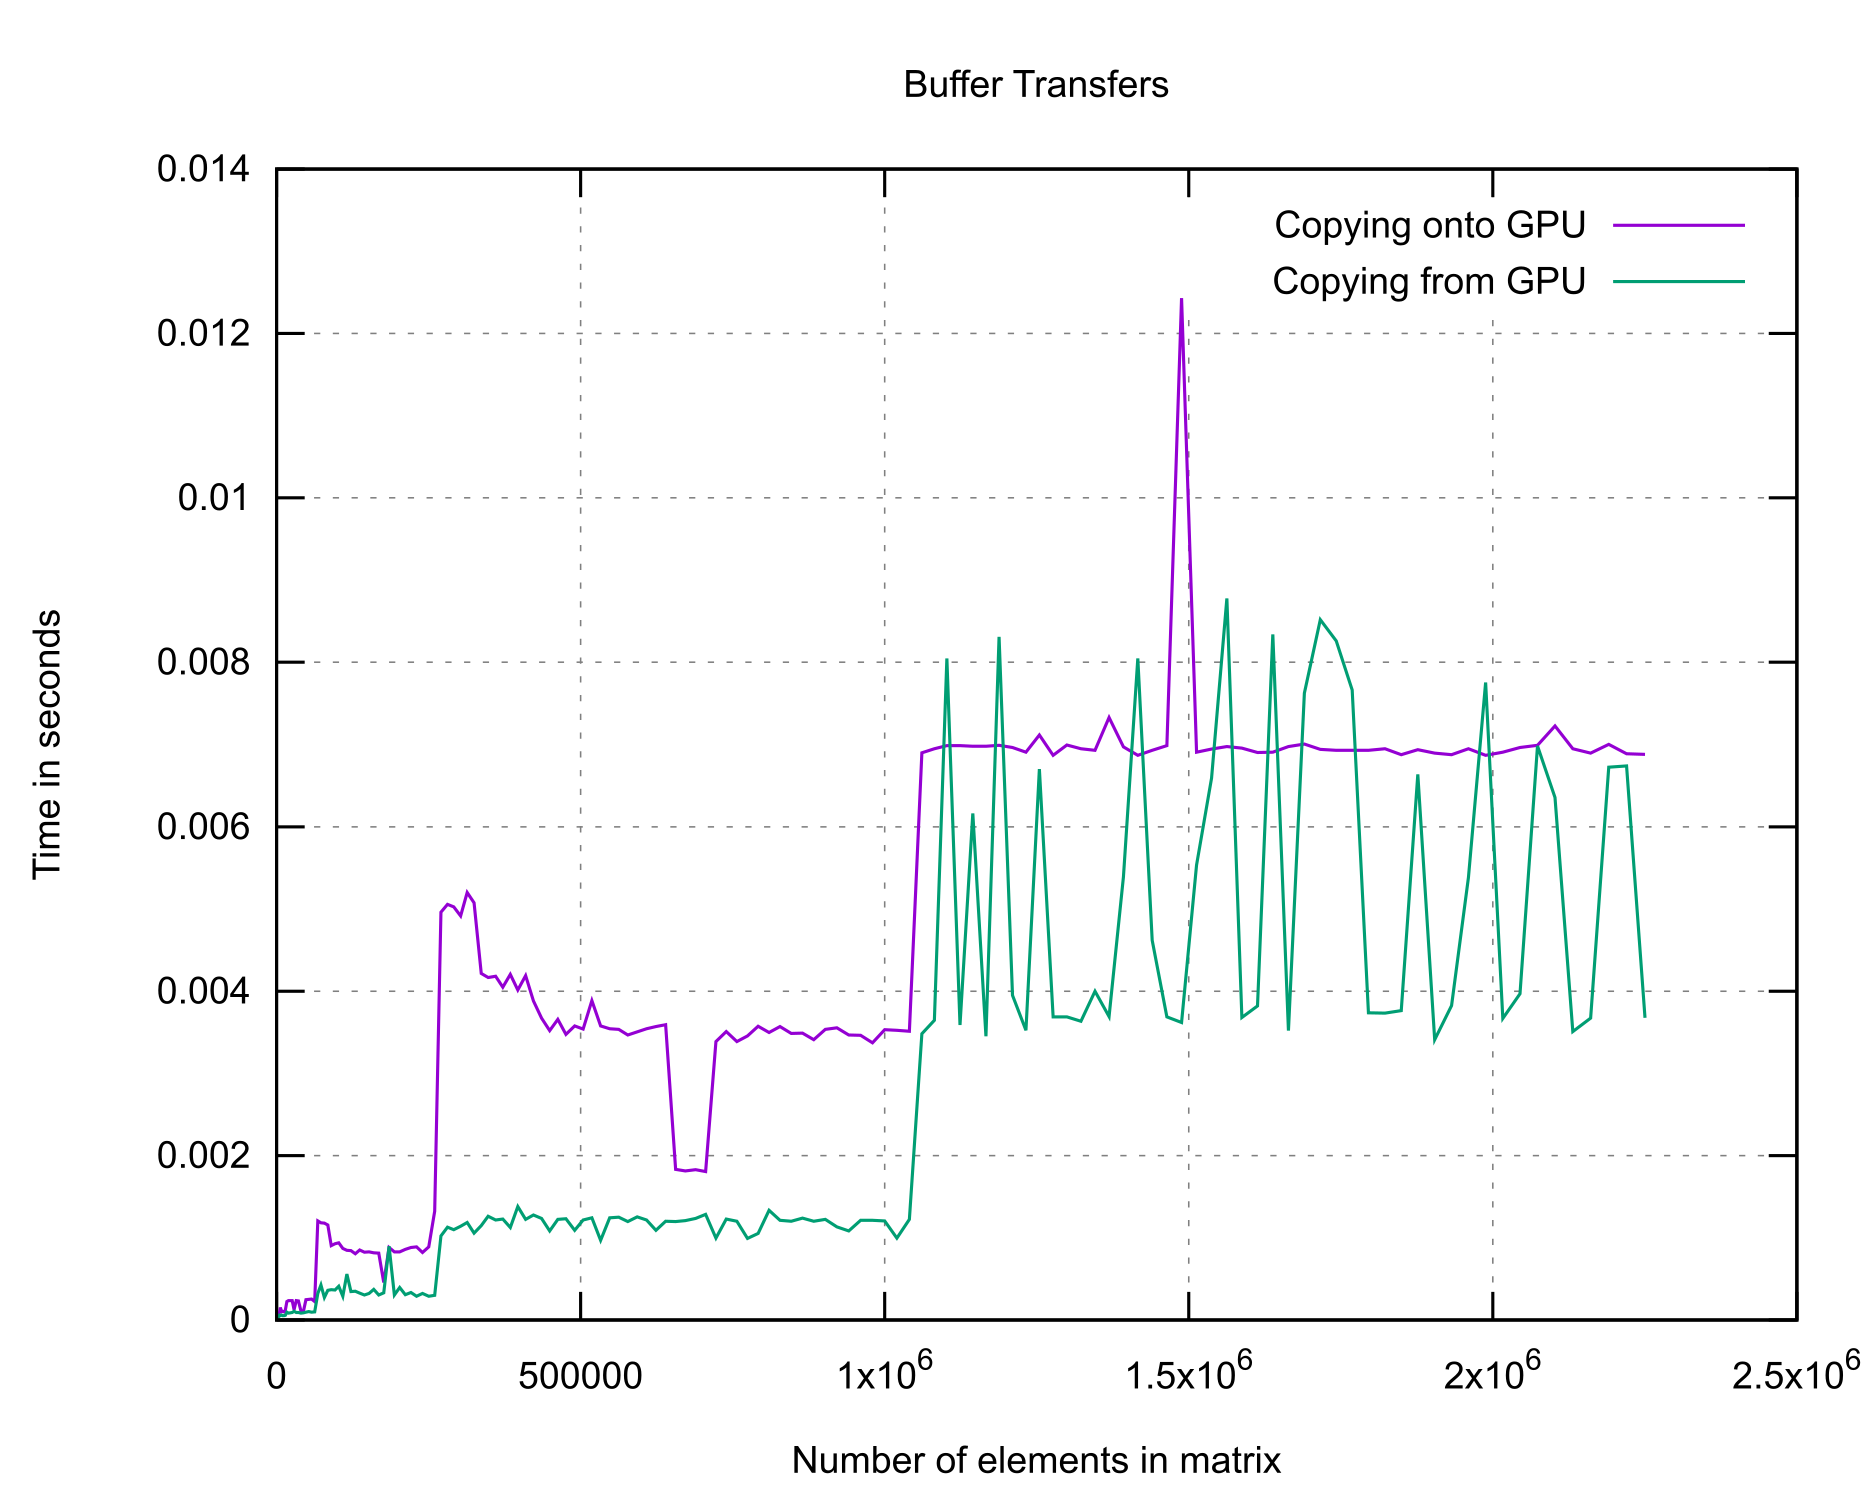
\includegraphics[width=\textwidth]{../resources/buffer_transfer.png}
\end{frame}

\begin{frame}
    \frametitle{Implémentation non naïve de la multiplication de matrices}
    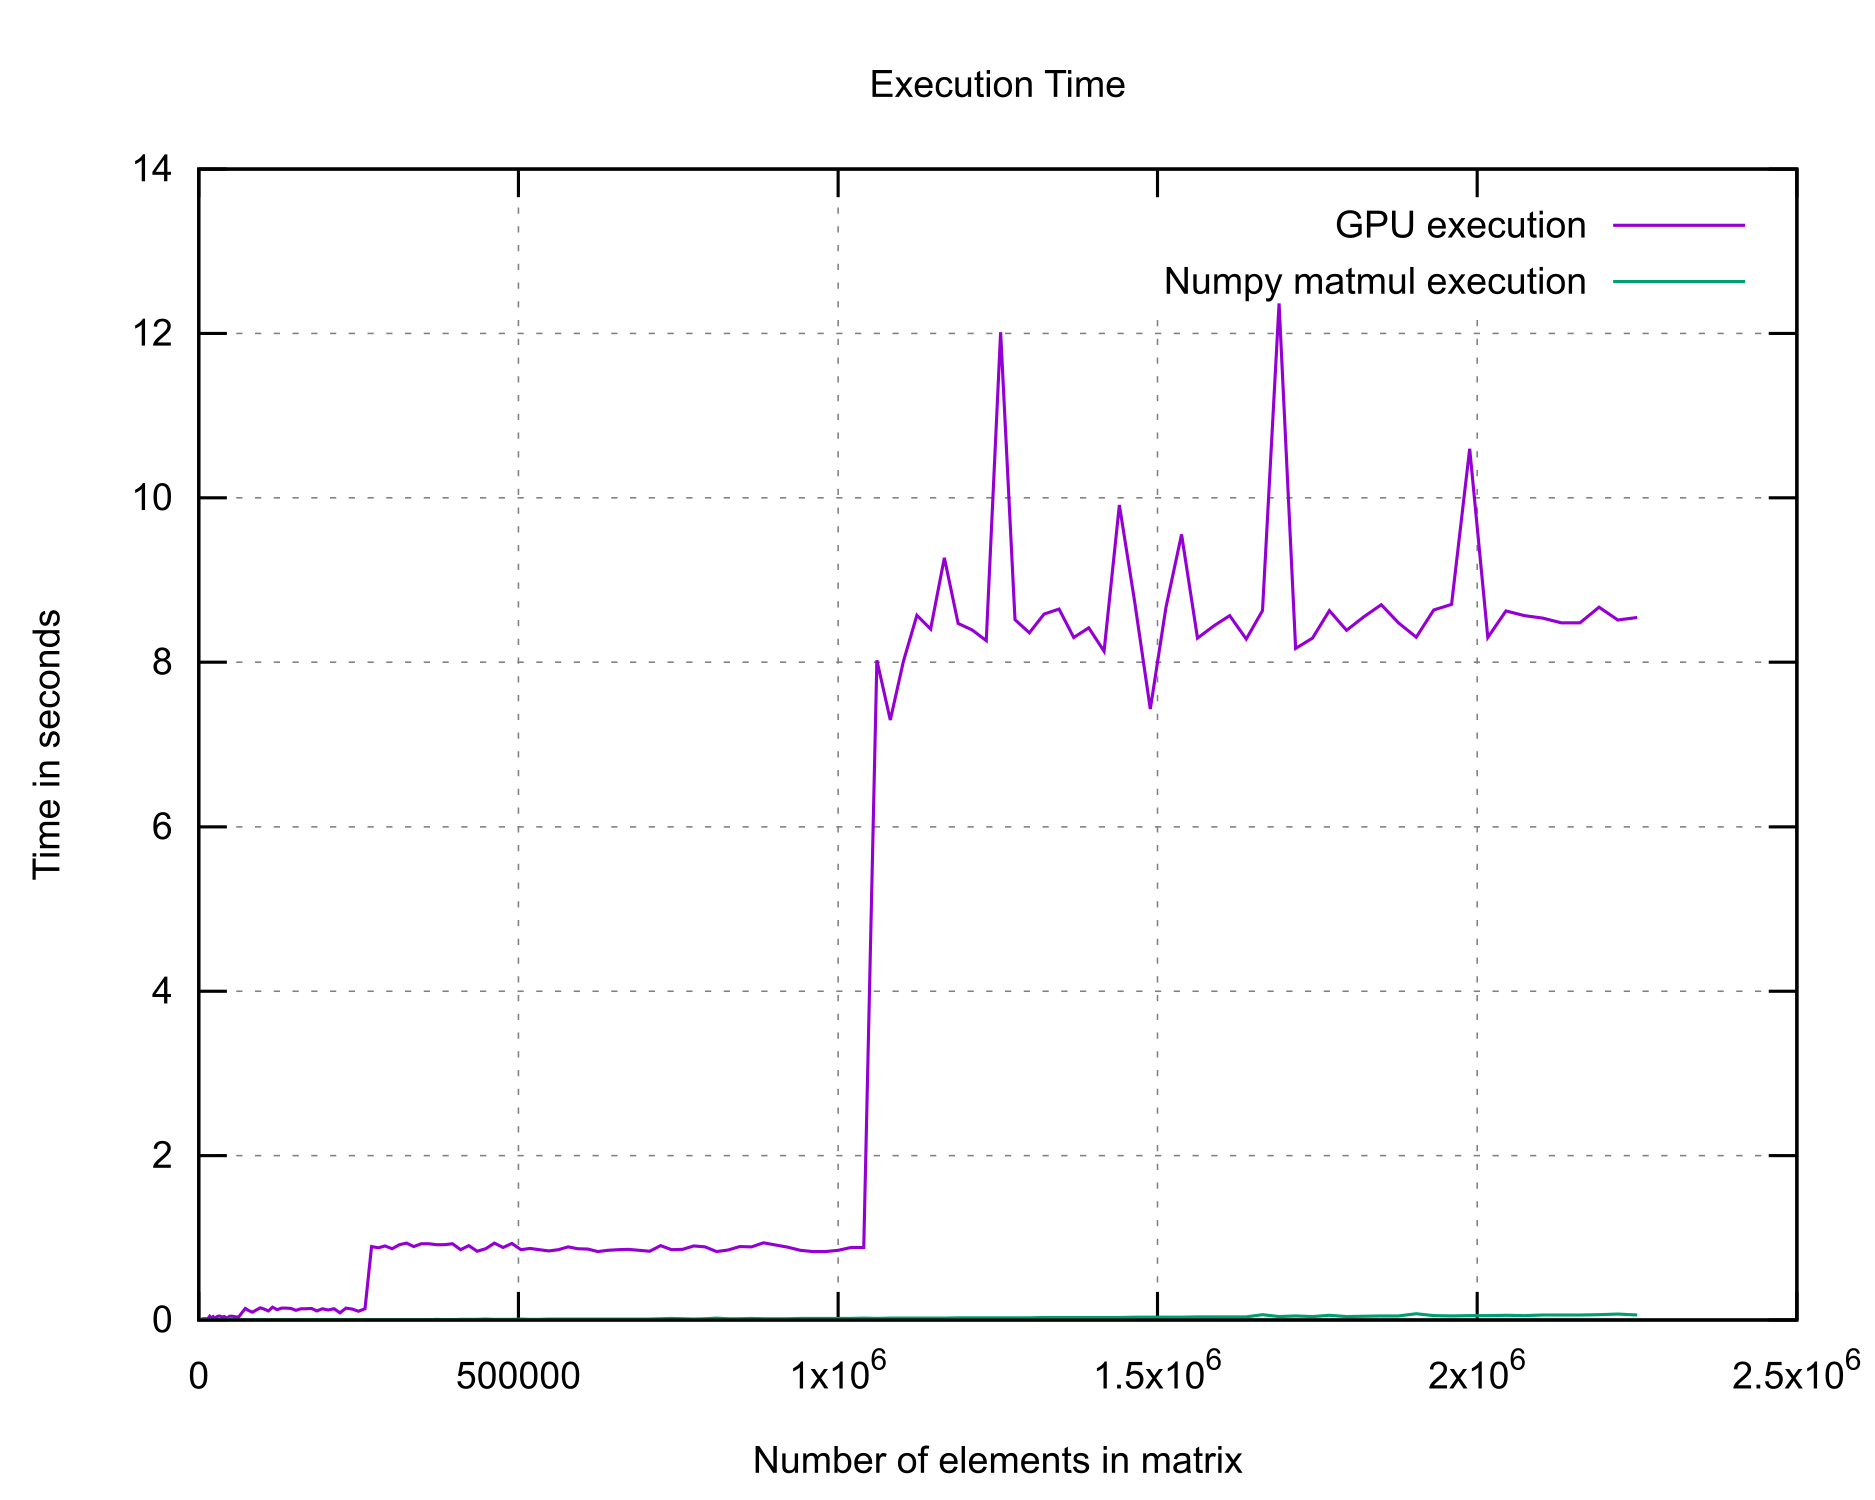
\includegraphics[width=\textwidth]{../resources/execution_time.png}
\end{frame}

\begin{frame}
    \frametitle{Implémentation non naïve de la multiplication de matrices}
    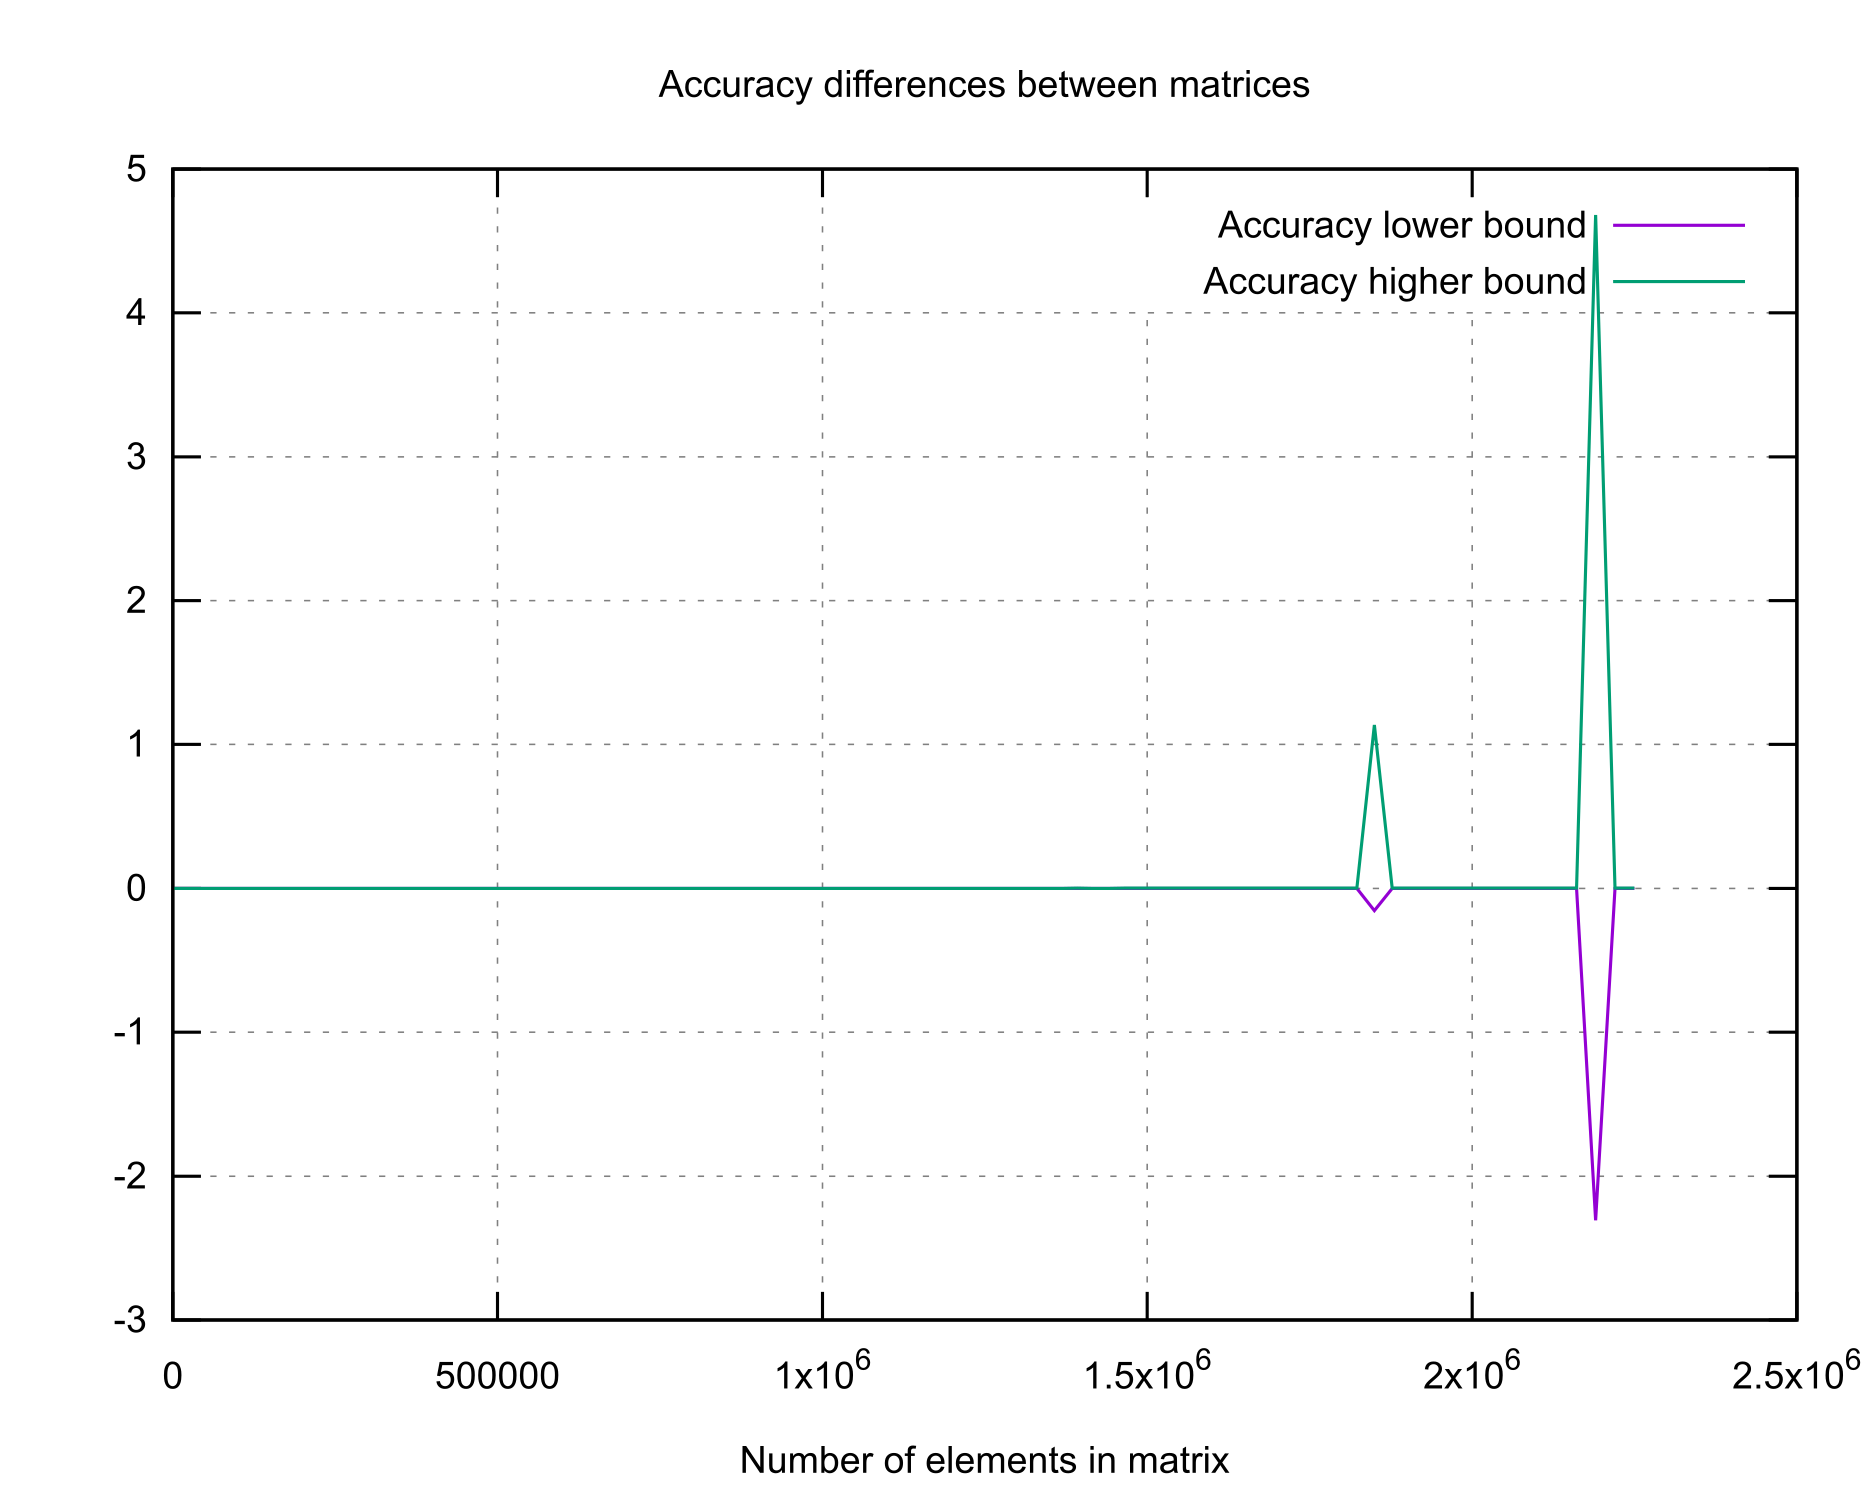
\includegraphics[width=\textwidth]{../resources/float_accuracy.png}
\end{frame}


\section{Conclusion}
\section{Conclusion}

\texttt{PyOpenCL} est un \textit{framework} simple d'utilisation et de prise en main 
avec une documentation officielle explicite. À l'opposé,
\texttt{OpenCL} est un language complexe. Beaucoup de notions tels que les 
modèles d'exécution et de mémoire sont à comprendre.
Même l'installation peut poser un challenge, il n'y a pas (pour \texttt{Intel}) 
de guide d'installation officiel expliquant l'ensemble des étapes. On n'a malheureusement 
pas réussi à ``le vendre'' car aucun de nos résultats n'ont été concluants. 
Cependant, il y a une raison pour laquelle \texttt{OpenCL} existe et que les
accélarations sur d'autres composants que le CPU est en essort. En imaginant qu'on 
arrive à obtenir des résultats concluants, il serait possible d'appliquer celà 
aux calculs complexes existants dans les réseaux de neurones par exemple afin 
de pouvoir accélérer l'apprentissage de l'intelligence artificielle. Dans tous 
les cas, il serait pratique pour envisager l'optimisation de \textit{bottlenecks}.
Cependant, il faut y réfléchir conséquemment avant car cela demande beaucoup 
d'investissement.


\end{document}
